% ============================================================
% Lectura_2_espanol_2col.tex
% Versión en español, 2 columnas (estilo IEEE) del paper:
% "GPU maps for the space of computation in triangular domain problems"
% Cristobal A. Navarro, Nancy Hitschfeld
% Universidad de Chile, 2014
%
% REGLAS DE TRADUCCIÓN APLICADAS:
% - Solo se traduce texto narrativo y títulos de secciones.
% - NO se traducen: fórmulas, variables, comandos LaTeX, etiquetas,
%   abreviaciones técnicas (BB, UTM, LTM, REC, RB, EDM, GPU, CUDA,
%   OpenCL), nombres de métodos, hardware, autores ni referencias.
% ============================================================

\documentclass[twocolumn,10pt,a4paper]{article}

% ----- Codificación y fuentes -----
\usepackage[utf8]{inputenc}
\usepackage[T1]{fontenc}
\usepackage{lmodern}

% Nota: babel[spanish] no instalado en esta TeX Live.
% Los acentos y ñ funcionan correctamente con inputenc+fontenc+lmodern.

% ----- Matemáticas -----
\usepackage{amsmath}
\usepackage{amssymb}
\usepackage{amsfonts}

% ----- Figuras y gráficos -----
\usepackage{graphicx}
\usepackage{float}
\usepackage{stfloats}   % permite figure* con [b] en 2 columnas

% ----- Tablas -----
\usepackage{booktabs}
\usepackage{array}

% ----- Referencias y citas -----
\usepackage{cite}
\usepackage{hyperref}

% ----- Márgenes estilo IEEE -----
\usepackage[top=1.8cm, bottom=2cm, left=1.5cm, right=1.5cm, columnsep=0.6cm]{geometry}

% ----- Otros -----
\usepackage{microtype}
\usepackage{abstract}
\renewcommand{\abstractnamefont}{\normalfont\bfseries}
\renewcommand{\abstracttextfont}{\normalfont\small\itshape}

% ============================================================
\title{\textbf{Mapas GPU para el espacio de cómputo\\en problemas de dominio triangular}}

\author{
  Cristobal A. Navarro\\
  {\small Departamento de Ciencias de la Computación, Universidad de Chile}\\
  {\small Centro de Estudios Cient\'ificos (CECs), Valdivia, Chile}\\
  {\small \texttt{crinavar@dcc.uchile.cl}}
  \and
  Nancy Hitschfeld\\
  {\small Departamento de Ciencias de la Computación, Universidad de Chile}\\
  {\small \texttt{nancy@dcc.uchile.cl}}
}

\date{}

% ============================================================
\begin{document}

% Título y abstract en una sola columna, luego empieza el 2-col
\twocolumn[{%
  \maketitle
  \begin{onecolabstract}
  Existe una etapa en el pipeline de cómputo de GPU donde una grilla de
  thread-blocks, o espacio de cómputo, es mapeada al dominio del problema.
  Normalmente, el espacio de cómputo es una bounding box (BB) $k$-dimensional
  que cubre un problema $k$-dimensional. Los threads que caen dentro del dominio
  del problema realizan cómputos y los que quedan fuera son descartados, todo
  ocurriendo en tiempo de ejecución. Para problemas con geometría no cuadrada,
  este enfoque hace que el espacio de cómputo sea mayor de lo necesario,
  desperdiciando muchos threads. Nuestro caso de interés son los problemas de
  dominio triangular bidimensional, alias \emph{td-problems}, donde casi la
  mitad del espacio de cómputo es innecesaria cuando se usa el enfoque BB.
  Problemas como el mapa de distancias euclidianas o la detección de colisiones
  son td-problems y aparecen frecuentemente como parte de un problema
  computacional mayor.

  En este trabajo, estudiamos varias funciones de mapeo y su contribución a un
  mejor espacio de cómputo mediante la reducción del número de threads
  innecesarios. Comparamos el rendimiento de cuatro estrategias de mapeo
  existentes: la bounding box (BB), el upper-triangular mapping (UTM), el
  rectangular box (RB) y la recursive partition (REC). Además, proponemos un
  mapa $g(\lambda)$ que mapea cualquier bloque $\lambda$ a una ubicación única
  $(i, j)$ en el dominio triangular. El mapeo se basa en las propiedades de la
  matriz triangular inferior y funciona en el espacio de bloques. La mejora
  teórica $I$ obtenida al usar $g(\lambda)$ está acotada superiormente como
  $I < 2$ y el número de bloques innecesarios se reduce de $O(n^2)$ a $O(n)$.
  Los resultados experimentales usando diferentes GPUs Nvidia Kepler muestran
  que para el cómputo de la matriz de distancias euclidianas, $g(\lambda)$
  logra una mejora de hasta 18\% sobre la estrategia básica de bounding box
  (BB), es más rápida que las estrategias UTM y REC, y casi tan rápida como
  RB. Los resultados de rendimiento en la detección de colisiones 3D con
  memoria compartida muestran que $g(\lambda)$ es el mapa más rápido de todos,
  y el único capaz de superar al enfoque de fuerza bruta (BB) por un margen de
  hasta 7\%. Estos resultados nos hacen comprender que una de las principales
  ventajas de $g(\lambda)$ es que usa mapeo en espacio de bloques, donde los
  valores de coordenadas son pequeños en magnitud y la organización de threads
  no se ve comprometida, haciendo el mapa estable en rendimiento bajo diferentes
  patrones de acceso a memoria.
  \end{onecolabstract}
  \vspace{0.4cm}
}]

% ============================================================
\section{Introducción}
\label{sec:introduction}

La computación en GPU es sin duda un área de investigación bien establecida
\cite{ref14,ref11,ref2}, desde el lanzamiento de plataformas de propósito
general como CUDA \cite{ref12} y OpenCL \cite{ref7}. En el modelo de
programación GPU de CUDA existen tres construcciones que permiten la ejecución
de algoritmos altamente paralelos: (1) thread, (2) block y (3) grid. Los
threads son los elementos más pequeños y se encargan de ejecutar las
instrucciones del kernel de GPU. Un block es una estructura intermedia que
contiene un conjunto de threads organizados en un espacio euclídeo. Los blocks
proporcionan acceso rápido a memoria compartida así como sincronización para
todos sus threads. El grid es la construcción más grande de la GPU y se encarga
de mantener todos los blocks juntos, organizados espacialmente para toda la
ejecución del kernel. Estas tres construcciones juegan un papel importante
cuando se mapea los recursos de ejecución al dominio del problema, y también
son necesarias para que la GPU programe y distribuya el trabajo correctamente
entre sus clusters de núcleos de procesamiento. OpenCL elige nombres
diferentes para estas construcciones: (1) work-element, (2) work-group y (3)
work-space, respectivamente.

Para cada aplicación GPU, existe una etapa en la que el grid, o espacio de
cómputo, se mapea a un dominio de problema para una eventual computación
posterior. Este mapa puede definirse como una función
$f(\mathbf{x}) : \mathbb{R}^k \rightarrow \mathbb{R}^p$
que transforma cada punto $k$-dimensional
$\mathbf{x} = (x_1, x_2, \ldots, x_k)$ de la grilla a un punto único
$p$-dimensional del dominio del problema. En otras palabras, $f(\mathbf{x})$
mapea el espacio de cómputo al dominio del problema.

Cuando el dominio del problema es simple en forma, las grillas rectangulares o
cuadradas son buenas elecciones porque la bounding box se ajusta perfectamente
al dominio. Las grillas rectangulares o cuadradas son las más utilizadas y se
caracterizan por usar el mapa de estrategia de bounding box (BB), donde
$f(\mathbf{x}) = \mathbf{x}$.

Sin embargo, otros problemas no se ajustan a un dominio con forma de caja
porque tienen una geometría diferente. Por ejemplo, algunos problemas 2D tienen
un dominio con forma triangular. Denominamos a este tipo de problemas
triangular-domain-problems o simplemente \emph{td-problems}. Construir una
grilla cuadrada para un td-problem no es la mejor elección porque genera
thread-blocks innecesarios que necesitarían ejecutar condicionales
\texttt{if-else} para descartarse, lo que conduce a una penalización en el
rendimiento. El escenario se ilustra en la Figura~\ref{fig:fig1}, donde los
blocks innecesarios están pintados con una carita roja triste.

\begin{figure}[H]
  \centering
  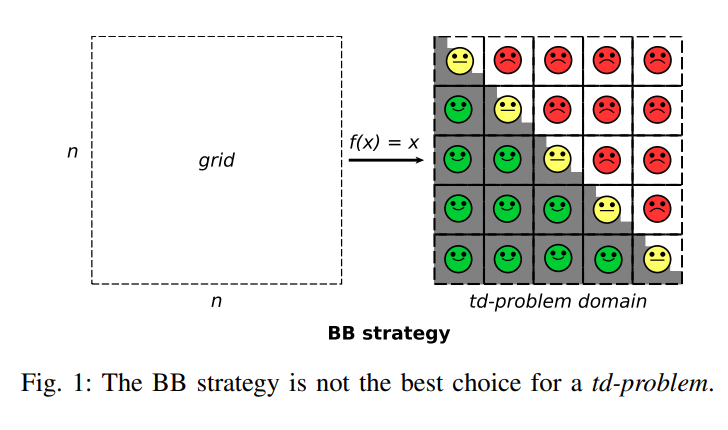
\includegraphics[width=\columnwidth]{figures/fig1.png}
  \caption{La estrategia BB no es la mejor elección para un \emph{td-problem}.}
  \label{fig:fig1}
\end{figure}

En este trabajo abordamos la falta de comparaciones entre diferentes estrategias
de mapeo existentes para td-problems, presentando resultados de rendimiento
ejecutando las mismas pruebas bajo el mismo hardware. La idea es establecer un
benchmark común para todas las estrategias de mapeo, usando tres diferentes
GPUs, y medir su rendimiento bajo tres casos: (1) dummy kernel, (2) matriz de
distancias euclidianas y (3) detección de colisiones. Hemos elegido estos tres
problemas porque representan diferentes escenarios: (1) kernel muy pequeño, (2)
patrones de memoria global y (3) patrones de memoria compartida. Además de este
benchmark, presentamos un nuevo mapa $g(\lambda)$, que funciona en el espacio
de bloques y usa las propiedades de la matriz triangular inferior. El mapa
$g(\lambda)$ realiza básicamente tres contribuciones: (1) implementación más
simple que las otras estrategias, (2) mayor rango de la raíz cuadrada que en
UTM \cite{ref1} y (3) organización de threads por bloque sin comprometer.

El resto del manuscrito se organiza de la siguiente manera: la
Sección~\ref{sec:related} presenta trabajos relacionados sobre mapas GPU. La
Sección~\ref{sec:blockwise} cubre la formulación de $g(\lambda)$. Los detalles
sobre su implementación y cómo elegimos la función de raíz cuadrada más rápida
están en la Sección~\ref{sec:implementation}. En la
Sección~\ref{sec:experiments} presentamos los resultados de rendimiento para
todas las estrategias existentes usando tres diferentes GPUs Nvidia Kepler: (1)
GTX~765M, (2) GTX~680 y (3) Tesla~K40. Finalmente, en la
Sección~\ref{sec:conclusions} concluimos discutiendo los puntos principales de
nuestro trabajo.

% ============================================================
\section{Trabajos Relacionados}
\label{sec:related}

El problema de mejorar el espacio de cómputo para td-problems es ciertamente
importante porque cualquier contribución al respecto beneficiará eventualmente,
por consecuencia, a todos los problemas de esta clase. Muchos problemas
computacionales son de hecho td-problems: mapas de distancias euclidianas (EDM)
\cite{ref10,ref8,ref9}, detección de colisiones \cite{ref1}, recorrido de
grafos a través de matrices de adyacencia \cite{ref6}, Autómatas Celulares
(por ejemplo, el Juego de la Vida de John Conway \cite{ref3}) en dominios
triangulares, inversión de matrices \cite{ref16}, descomposición LU/Cholesky
\cite{ref4}, entre otros.

En el campo de los mapas de distancias, Ying et al.\ han propuesto una
implementación GPU para el cómputo paralelo de distancias de secuencias de
ADN \cite{ref17}, que se basa en EDM. En su trabajo, los autores mencionan
que el dominio del problema es ciertamente simétrico y reconocen que solo la
parte triangular superior o inferior de la matriz de interacción requiere
cómputo. Li et al.\ \cite{ref8} también han trabajado en EDMs basados en GPU
para grandes conjuntos de datos y también han identificado la simetría
involucrada en el cómputo. Sin embargo, en ambos trabajos no hay mención del
mapeo del espacio de cómputo.

Jung et al.\ \cite{ref5} propusieron en 2008 estructuras de datos compactas
para representar matrices triangulares y simétricas con aplicaciones a la
descomposición LU y Cholesky \cite{ref4}. La estrategia se basa en construir
una estrategia de rectangular box (RB) para acceder y almacenar una matriz
triangular (superior o inferior). Las estructuras de datos se vuelven
prácticamente la mitad del tamaño respecto a los métodos clásicos basados en
la matriz completa. Originalmente, esta estrategia está orientada a la
estructura de memoria de la matriz, pero también puede aplicarse de manera
análoga al espacio de cómputo.

En 2009, Ries et al.\ contribuyeron con un método GPU paralelo para la
inversión de matrices triangulares \cite{ref16}. Los autores identifican que
el espacio de cómputo puede ciertamente mejorarse usando una recursive
partition (REC) de la grilla, basada en una estrategia de divide y vencerás.

En 2012, Q.~Avril et al.\ propusieron una función de mapeo GPU para la
detección de colisiones basada en las propiedades del mapa triangular superior
\cite{ref1}. El mapa, denominado UTM, es una función
$f(k) \rightarrow (a, b)$, donde $k$ es el índice lineal de un thread $t_k$
y el par $(a, b)$ es una coordenada bidimensional única en la matriz
triangular superior. Los autores mencionan que para el cómputo de la raíz
cuadrada usan la aproximación de raíz cuadrada rápida de Carmack y Lomont
(basada en el algoritmo de aproximación de Newton-Raphson \cite{ref15}) para
acelerar la función de mapeo. Los errores de aproximación se corrigen
usando dos instrucciones condicionales dentro del kernel. Su implementación
de raíz cuadrada $\sqrt{x}$ es precisa para $x \in [0, 100M]$, lo que según
su función de mapeo se referiría a problemas en el rango $N \in [0, 3000]$.

Hasta la fecha, no ha habido una comparación dedicada de las diferentes
estrategias propuestas para mejorar el espacio de cómputo en td-problems. En
el mejor caso podemos encontrar una comparación entre el mapa de Avril y la
estrategia BB \cite{ref1}, donde los autores reportan un speedup de casi 2X,
sin embargo, el filtrado se realiza por ID de thread en lugar de por
coordenadas de bloque, lo que hace al mapa BB más lento.

El mapa triangular aún puede mejorarse para funcionar con tamaños de problema
de $N < 30000$ y también para poder usar la memoria compartida de la GPU,
a través de una formulación por bloques.

% ============================================================
\section{El Mapa Triangular por Bloques}
\label{sec:blockwise}

\subsection{Formulación}

Es importante distinguir primero entre dos tipos de mapeos que pueden
realizarse en la GPU: (1) mapeo por thread y (2) mapeo por bloque. El mapeo
por thread es donde cada thread usa su propio índice único como parámetro para
la función de mapeo, tal como en el mapa UTM \cite{ref1}. En el mapeo por
bloque, los threads usan su índice de bloque para mapearse todos a una
ubicación específica, seguido de un desplazamiento local según la posición
relativa en el bloque. Hemos elegido continuar con el mapeo por bloque y sus
ventajas se explican más adelante.

Sea $N$ el tamaño del problema (asumiendo elementos data-paralelos), $A$ un
td-problem de tamaño $N(N+1)/2$, $n = \lceil N/\rho \rceil$ el número de
bloques necesarios para cubrir los datos a lo largo de una dimensión y $\rho$
el número de threads por bloque por dimensión, o tamaño de bloque dimensional
(por simplicidad, asumimos que todas las dimensiones son iguales). Una
estrategia BB simplemente construiría una grilla cuadrada, denominada $G_{BB}$,
de $n \times n$ bloques y pondría instrucciones condicionales para cancelar los
cómputos fuera del dominio del problema. Un análisis más fino indica que
$n(n+1)/2$ bloques son suficientes para cubrir el dominio del problema de $A$:

\begin{equation}
A = \left|
\begin{array}{ccccc}
0 & & & & \\
1 & 2 & & & \\
3 & 4 & 5 & & \\
\cdots & \cdots & \cdots & \cdots & \\
\dfrac{n(n-1)}{2} & \dfrac{n(n-1)}{2}+1 & \cdots & \cdots & \dfrac{n(n+1)}{2}-1
\end{array}
\right|
\label{eq:A}
\end{equation}

\textit{Nota}: para el resto del artículo nos referiremos a nuestro enfoque
de mapeo como LTM por \emph{lower triangular mapping}, o simplemente
$g(\lambda)$.

La idea es construir una grilla bidimensional balanceada $G_{LTM}$ que cubra
la matriz triangular inferior, usando solamente $n(n+1)/2$ bloques. Por grilla
balanceada entendemos $n' = \lceil\sqrt{n(n+1)/2}\rceil$ bloques por
dimensión. La Figura~\ref{fig:fig2} ilustra $G_{LTM}$ y cómo es más pequeña
que $G_{BB}$ de la Figura~\ref{fig:fig1}, mientras aún proporciona el número
necesario de bloques para cubrir el dominio del problema. El resultado es una
reducción de $n(n-1)/2 \in O(n^2)$ a $n/2 \in O(n)$ bloques innecesarios.

\begin{figure}[H]
  \centering
  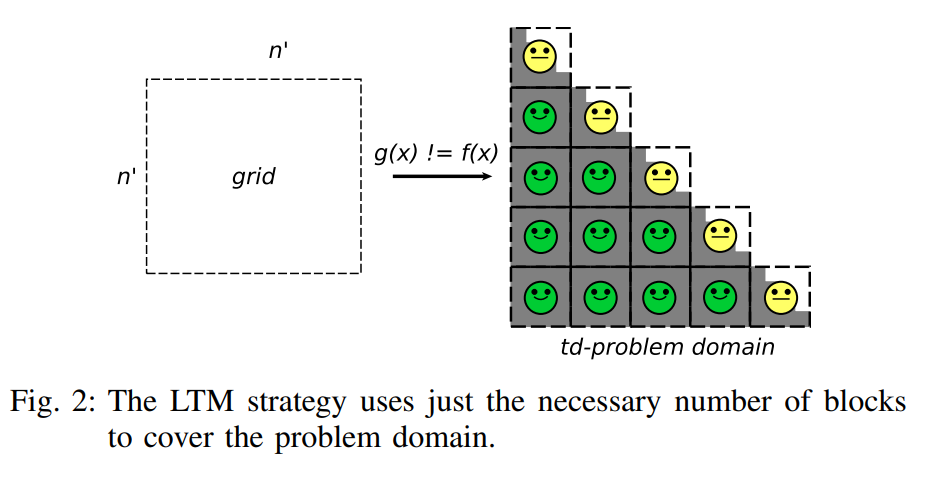
\includegraphics[width=\columnwidth]{figures/fig2.png}
  \caption{La estrategia LTM usa solo el número necesario de bloques para
           cubrir el dominio del problema.}
  \label{fig:fig2}
\end{figure}

El siguiente paso es formular $g(\lambda) = (i, j)$ donde $(i, j)$ son las
coordenadas en el espacio del problema y $\lambda$ es el índice del bloque
$B_{x,y}$ calculado como $\lambda = x + yn'$ en el espacio de bloques.

\textbf{Teorema 1}: Para cualquier bloque $B_{x,y}$ con $\lambda = x + yn'$,
su función de mapeo $g(\lambda)$ es:
\begin{equation}
g(\lambda) = (i, j) = \left(
  \left\lfloor \sqrt{\tfrac{1}{4} + 2\lambda} - \tfrac{1}{2} \right\rfloor,
  \; \lambda - i(i+1)/2
\right)
\label{eq:g_lambda}
\end{equation}

\textit{Demostración}: El índice $\lambda$ puede expresarse como un número
triangular con un límite de suma desconocido $x$:
\begin{equation}
\lambda = \sum_{k=1}^{x} k
\label{eq:triangular}
\end{equation}

El índice del bloque más a la izquierda que se encuentra en la misma fila del
bloque $\lambda$-ésimo corresponde a la suma en el rango $[1, i]$.
Similarmente, el índice del bloque más a la izquierda de la fila $(i+1)$-ésima
es una suma en el rango $[1, i+1]$. Para todos los índices $\lambda$ bajo la
misma fila $i$, el rango de la sumatoria se encuentra en un rango
$[1, i+\epsilon]$, donde $\epsilon < 1$:
\begin{equation}
\sum_{k=1}^{i} k \leq \lambda = \sum_{k=1}^{i+\epsilon} k < \sum_{k=1}^{i+1} k
\label{eq:sum_bounds}
\end{equation}

Por lo tanto $x \in \mathbb{R}$ e $i = \lfloor x \rfloor$. Como
$\sum_{k=1}^{x} k = x(x+1)/2$, $x$ se encuentra simplemente resolviendo una
ecuación de segundo grado con coeficientes $a = 1$, $b = 1$ y $c = -2$:
\begin{equation}
x^2 + x - 2\lambda = 0
\label{eq:quadratic}
\end{equation}

La solución de interés es:
\begin{equation}
x = \frac{\sqrt{1 + 8\lambda} - 1}{2} = \sqrt{\tfrac{1}{4} + 2\lambda} - \tfrac{1}{2}
\label{eq:x_solution}
\end{equation}

Y la coordenada $i$ del bloque $\lambda$-ésimo se calcula como:
\begin{equation}
i = \lfloor x \rfloor = \left\lfloor \sqrt{\tfrac{1}{4} + 2\lambda} - \tfrac{1}{2} \right\rfloor
\label{eq:i_coord}
\end{equation}

La coordenada $j$ es la distancia desde el bloque $\lambda$-ésimo hasta el
bloque más a la izquierda en la misma fila:
\begin{equation}
j = \lambda - \frac{i(i+1)}{2}
\label{eq:j_coord}
\end{equation}

Si la diagonal no es necesaria, entonces $g(\lambda)$ se convierte en:
\begin{equation}
g(\lambda) = (i, j) = \left(
  \left\lfloor \sqrt{\tfrac{1}{4} + 2\lambda} + \tfrac{1}{2} \right\rfloor,
  \; \lambda - i(i+1)/2
\right)
\label{eq:g_no_diag}
\end{equation}

Al comparar LTM con su contraparte más cercana UTM \cite{ref1}, identificamos
tres mejoras: (1) $g(\lambda)$ usa menos operaciones de punto flotante que en
UTM ya que usa el mapeo triangular inferior. (2) LTM mapea bloques y no threads
como en UTM. Como $g(\lambda)$ es un mapa de bloques y el número de bloques
es $n = N/\rho$, la raíz cuadrada da errores de aproximación más pequeños,
permitiendo un cómputo preciso para valores más grandes de $N$. (3) La
organización de threads no se ve comprometida en LTM, mientras que en UTM sí.

\subsection{Cotas del factor de mejora}

La reducción de bloques innecesarios de $O(n^2)$ a $O(n)$ podría sugerir que
la mejora podría alcanzar en el mejor caso un factor de 2X. Para que esto sea
posible, habría que medir solo el tiempo de mapeo, de modo que los bloques
necesarios e innecesarios hagan los mismos trabajos, y asumir que la función
de mapeo $g(\lambda)$ es tan barata como en la estrategia BB. En el siguiente
análisis analizamos el factor de mejora considerando un escenario más realista
donde $g(\lambda)$ tiene un costo mayor que el mapa BB, debido al cómputo de
la raíz cuadrada involucrado.

La estrategia LTM depende fuertemente de la raíz cuadrada que en teoría es
asintóticamente $O(M(n))$ \cite{ref18}, donde $M(n)$ es el costo de
multiplicar dos números de $n$ dígitos. Considerando que los números reales se
representan por un número finito de dígitos (es decir, números de punto
flotante con un máximo de $m$ dígitos), entonces todas las operaciones básicas
cuestan una cantidad fija de tiempo, llevando a un costo constante
$M(m) = C_s \in O(1)$. Todos los demás cómputos son operaciones aritméticas
elementales y se tomarán como un costo adicional de $C_a \in O(1)$. La
estrategia LTM tiene un costo de $\tau = C_s + C_a = O(1)$ para cada thread
mapeado. Por otro lado, la estrategia BB verifica para cada thread si
$B_y \leq B_x$ para continuar o no, también resultando en un costo constante
de $\beta \in O(1)$.

Para este caso particular, el análisis asintótico no da información precisa
sobre el factor de mejora, ya que tanto LTM como BB se encuentran en el mismo
orden de complejidad (es decir, $n(n+1)/2 \in O(n^2)$), por lo tanto la
mejora debería ser un factor constante. Procedemos a un análisis no asintótico
más fino para encontrar las constantes involucradas en el factor de mejora.

Sean $|G_{BB}|$ y $|G_{LTM}|$ el número de bloques para las estrategias BB y
LTM, respectivamente, y $\rho$ el número de threads por bloque por dimensión
como se mencionó antes. Es evidente que $\beta$ es más barato que $\tau$, por
lo tanto $\tau = k\beta$ con una constante $k \geq 1$. El factor de mejora $I$
se puede obtener dividiendo el costo total de BB por LTM en sus grillas
completas:

\begin{equation}
I = \frac{\beta |G_{BB}| \rho^2}{\tau |G_{LTM}| \rho^2} =
    \frac{\beta n^2}{\tau n(n+1)/2} =
    \frac{2\beta n^2}{\tau n^2 + \tau n}
\label{eq:improvement}
\end{equation}

Como se muestra en (\ref{eq:improvement}), la mejora no depende de los
threads, sino de los bloques. Para $n$ grande tenemos:
\begin{equation}
I = \frac{2\beta n^2}{\tau n^2 + \tau n} \approx \frac{2\beta}{\tau}
\label{eq:improvement_large}
\end{equation}

Si $\tau \geq 2\beta$, el rendimiento es igual o peor que el de BB.
Una mejora real se logra cuando:
\begin{equation}
\beta \leq \tau < 2\beta
\label{eq:real_improvement}
\end{equation}

Usando la relación $\tau = k\beta$ en (\ref{eq:improvement_large}) obtenemos:
\begin{equation}
I \approx 2/k
\label{eq:I_approx}
\end{equation}

Como $k > 1$, el rango de $I$ es:
\begin{equation}
0 < I < 2
\label{eq:I_range}
\end{equation}

Cualquier valor en el rango $1 < I < 2$ significa una mejora en el rendimiento
y un valor en el rango $0 < I < 1$ significará una ralentización respecto a la
estrategia BB. La constante $k$ puede interpretarse como el costo y la
sobrecarga de la función de mapeo. Un valor de $k \approx 1$ significa que se
logra la máxima mejora posible: $I_{max} \approx 2$, para $n$ grande. En
la práctica, un valor de $k \approx 1$ es demasiado optimista y no ocurriría.
Nuestra hipótesis es que el hardware real podría dar un valor en el rango
$1.5 \leq k < 2.0$, lo que correspondería a $1.00 < I \leq 1.33$. Cualquier
valor de $k \geq 2$ no llevará a ninguna mejora, resultando en un rendimiento
más lento que la estrategia BB. Es importante enfatizar que $C_a$ (operaciones
aritméticas) no tendrá mucho margen de optimización como $C_s$. Por lo tanto,
obtener el valor máximo posible de $I$ dependerá finalmente de qué tan rápida
pueda ser la raíz cuadrada.

% ============================================================
\section{Implementación de LTM}
\label{sec:implementation}

En esta sección elegimos la mejor de tres implementaciones de raíz cuadrada
para usar en el mapa LTM. También explicamos en términos generales la idea
detrás de las otras estrategias de mapeo que también hemos implementado para
una comparación posterior.

\subsection{Eligiendo la mejor raíz cuadrada}

El rendimiento de la estrategia LTM depende fuertemente de qué tan rápido sea
el cómputo del índice $i$. Más precisamente, del cómputo de la raíz cuadrada
como se mencionó antes. Realizamos tres versiones del mapa LTM, usando
diferentes implementaciones de raíz cuadrada, y calculamos el factor de mejora
con respecto a la estrategia BB. La primera, denominada LTM-X, usa la función
\texttt{sqrtf(x)} predeterminada de CUDA y es la más simple.

La segunda implementación de LTM, denominada LTM-N, calcula la raíz cuadrada
usando tres iteraciones del método de Newton-Raphson \cite{ref18,ref15}.
Usamos la implementación de Carmack y Lomont. Esta implementación ha demostrado
ser efectiva para aplicaciones que permiten pequeños errores. El valor inicial
usado es el número mágico \texttt{0x5f3759df} (esta suposición inicial se
conoció cuando \textit{Id Software} publicó el código fuente de Quake~3 en el
año 2005). Hemos encontrado que agregar una constante de
$\epsilon = 10^{-4}$ al resultado de la raíz cuadrada puede corregir errores
de aproximación en el rango $N \in [0, 30720]$.

La tercera implementación, denominada LTM-R, usa la raíz cuadrada recíproca
implementada en hardware, \texttt{rsqrtf(x)}:
\begin{equation}
\sqrt{x} = \frac{x}{\sqrt{x}} = x \cdot \texttt{rsqrtf}(x)
\label{eq:rsqrt}
\end{equation}

En términos de simplicidad, LTM-R es similar a LTM-X, la única diferencia es
que agrega $\epsilon = 10^{-4}$ al final para corregir errores de aproximación,
igual que en LTM-N.

Medimos el factor de mejora de cada implementación con respecto a la estrategia
BB ejecutando un dummy kernel que calcula los índices $i$, $j$ y escribe la
suma $i + j$ en una ubicación constante de memoria. Es necesario realizar al
menos un acceso a memoria; de lo contrario, el compilador puede optimizar el
código eliminando parte del costo del mapeo. La Figura~\ref{fig:fig3} muestra
el factor de mejora como $I = BB/LTM$ usando las tres diferentes
implementaciones, ejecutándose en tres diferentes GPUs Nvidia Kepler: GTX~680,
GTX~765M y Tesla~K40. Hemos incluido el mapa BB como referencia, como una
línea negra horizontal en $I = 1$. En el lado derecho de la
Figura~\ref{fig:fig3} comparamos el número de bloques innecesarios entre BB
y LTM.

De los resultados, observamos que LTM-X es más lento que BB cuando se ejecuta
en el GTX~680 y GTX~765M, alcanzando $I_{680} \approx 0.87$ y
$I_{765M} \approx 0.83$, respectivamente. Para las mismas dos GPUs, LTM-N
logra una mejora de $I_{680} \approx 1.025$ e $I_{765M} \approx 0.96$, que
es prácticamente el rendimiento de BB. Por otro lado, LTM-R logra mejoras de
$I_{680} \approx 1.15$ e $I_{765M} \approx 1.1$. De estos resultados,
observamos que usar la raíz cuadrada inversa es la mejor opción para el
GTX~680 y GTX~765M. Para el caso del Tesla~K40, observamos que las tres
implementaciones logran una mejora de $I_{K40} \approx 1.08$, lo que permite
elegir LTM-X sin ninguna penalización en el rendimiento.

% Fig 3 ocupa ambas columnas (figura ancha)
\begin{figure*}[t]
  \centering
  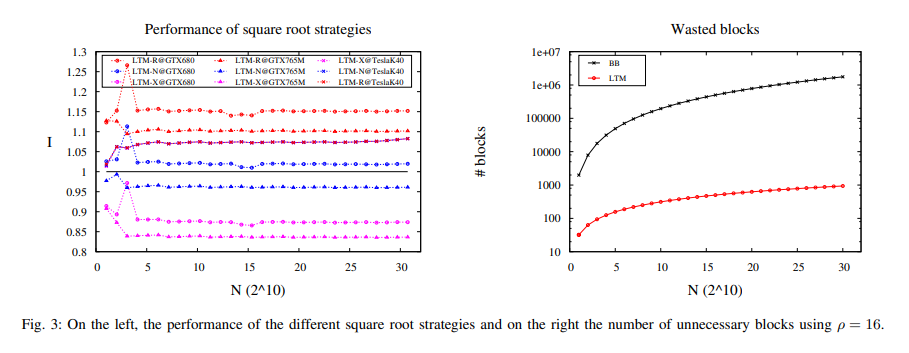
\includegraphics[width=\textwidth]{figures/fig3.png}
  \caption{A la izquierda, el rendimiento de las diferentes estrategias de
           raíz cuadrada, y a la derecha el número de bloques innecesarios
           usando $\rho = 16$.}
  \label{fig:fig3}
\end{figure*}

\subsection{Implementando las otras estrategias}

Hemos implementado las otras estrategias de mapeo: BB, RB, REC y UTM
siguiendo los detalles proporcionados por los autores \cite{ref5,ref1,ref16}.
A cada implementación agregamos la siguiente restricción: el mapa no puede usar
ninguna memoria que crezca como función de $N$. Esto significa que no se
permiten arreglos auxiliares como tablas de búsqueda; sin embargo, las
constantes sí están permitidas. Impusimos esta restricción para garantizar que
la memoria de GPU esté dedicada al problema de la aplicación.

Para la estrategia de bounding box (BB), los bloques sobre la diagonal son
descartados en tiempo de ejecución, sin necesidad de calcular una coordenada
de thread. Esto se hace verificando si $B_x > B_y$ para cada thread. Para
el resto de los threads, se calcula la coordenada. La condición $i > j$ aún
se realiza para descartar threads en bloques donde $B_x = B_y$. Esta
implementación de BB es más rápida que calcular primero la coordenada del
thread y filtrar después.

La estrategia de rectangular box (RB) se basa en el trabajo de Jung et al.\
\cite{ref5}. Este método toma la porción sub-triangular de los threads donde
$t_x > N/2$, la rota CCW y la coloca sobre la diagonal para formar una grilla
rectangular (ver Figura~\ref{fig:fig4}). El trabajo original era en realidad
una técnica de empaquetado de memoria orientada a las estructuras de datos y
no un mapa GPU, sin embargo la idea principal de la estrategia es adecuada
como función de mapeo. Eliminamos la textura de búsqueda usada en la
implementación original y realizamos el mapeo de coordenadas aritméticamente
en tiempo de ejecución. Todos los threads por debajo de la diagonal solo
necesitan mapearse a $i = t_y - 1$, mientras que $j$ permanece igual. Los
threads en o sobre la diagonal se mapean a $i = N - t_y - 1$ y
$j = N - i - 1$. Este mapeo es para valores pares de $N$. El caso de $N$ impar
es la misma idea pero particionando en $\lfloor N/2 \rfloor$. Una
característica notable del mapa RB es que el número de bloques innecesarios
es asintóticamente $O(1)$.

La estrategia de recursive partition (REC) fue propuesta para la GPU
\cite{ref16} para la inversión de matrices. En este método, el tamaño del
problema se define como $N = m \cdot 2^k$, donde $k$ y $m$ son enteros
positivos y $m$ es múltiplo de $\rho$ (el tamaño de bloque). La idea es hacer
una recursión binaria bottom-up de $k$ niveles, similar al merge-sort (ver
Figura~\ref{fig:fig4}). En cada nivel, se lanza una grilla de bloques para
ejecución paralela, un total de $k$ veces. Este método requiere un pase
adicional para calcular los bloques en la diagonal. Más detalles sobre cómo
se construye la grilla y cómo se distribuyen los bloques están bien explicados
en \cite{ref16}. En el trabajo original, el mapeo de los bloques a sus
respectivas ubicaciones en cada nivel se logra usando una tabla de búsqueda
almacenada en memoria constante. En este trabajo, hacemos el mapeo en tiempo
de ejecución como en RB.

\begin{figure}[H]
  \centering
  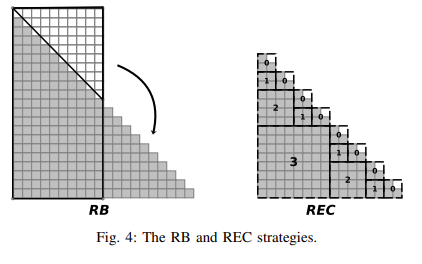
\includegraphics[width=0.85\columnwidth]{figures/fig4.png}
  \caption{Las estrategias RB y REC.}
  \label{fig:fig4}
\end{figure}

El upper-triangular mapping (UTM) fue propuesto por Avril et al.\ \cite{ref1}
para realizar detección de colisiones eficiente en la GPU. Este método es muy
similar a LTM; dado un tamaño de problema $N$ y un índice de thread $k$, su
par único $(a, b)$ se calcula como
$a = \left\lfloor
\frac{-(2n+1) + \sqrt{4n^2 - 4n - 8k + 1}}{-2}
\right\rfloor$ y
$b = (a+1) + k - \frac{(a-1)(2n-a)}{2}$. La estrategia UTM usa la idea de
mapear a la matriz triangular superior sin la diagonal. El mapeo a la matriz
triangular superior aún permite resolver
dominios con forma triangular inferior, y viceversa mediante transposición. Una
diferencia importante entre UTM y LTM es que UTM usa organización lineal de
threads y el mapa funciona en el espacio lineal de threads, donde se necesita
calcular números muy grandes en la raíz cuadrada. Por otro lado, LTM usa una
organización bidimensional de threads y el mapa funciona en el espacio lineal
de bloques, haciendo que la raíz cuadrada trabaje con números más pequeños que
los que usa UTM.

% ============================================================
\section{Resultados Experimentales}
\label{sec:experiments}

Nuestro diseño experimental consiste en medir el rendimiento de LTM y
compararlo contra todas las estrategias existentes: bounding box (BB),
upper-triangular mapping (UTM) \cite{ref1}, rectangular box (RB) \cite{ref5}
y recursive partition (REC) \cite{ref16}. Verificamos que las salidas para
cada estrategia fueran siempre correctas. Se realizan tres pruebas a cada
estrategia: (1) el dummy kernel, (2) EDM y (3) detección de colisiones. La
prueba (1) simplemente escribe la coordenada $(i, j)$ en una ubicación fija
de memoria. El propósito del dummy kernel es medir solo el costo de la
estrategia y no el costo del problema de la aplicación. La prueba (2) consiste
en calcular la matriz de distancias euclidianas (EDM) usando cuatro
características. El propósito es medir cuál es el rendimiento de todas las
estrategias al resolver un problema basado en memoria global. La prueba (3)
consiste en realizar la detección de colisiones de $N$ esferas con radio
aleatorio dentro de una caja unitaria. El objetivo de esta última prueba es
medir el rendimiento de los kernels usando un enfoque de memoria compartida.

La razón por la que elegimos estas pruebas es porque son suficientemente
simples para estudiar su rendimiento desde la perspectiva de un mapa GPU y
usan diferentes paradigmas de acceso a memoria, como memoria global y memoria
compartida. Basándonos en estos argumentos, esperamos que los resultados de
rendimiento obtenidos por las tres pruebas den información sobre cuál sería el
comportamiento para problemas más complejos que caen en uno de los dos
paradigmas de acceso a memoria. Además, decidimos ejecutar las pruebas en tres
GPUs diferentes para obtener métricas lo suficientemente generales que puedan
proporcionar patrones de rendimiento.

Los detalles del hardware y el número máximo de bloques simultáneos (sblocks)
para cada GPU se listan en la Tabla~\ref{tab:hardware}. Los resultados de
rendimiento para el dummy kernel, EDM y detección de colisiones en 1D/3D se
presentan en la Figura~\ref{fig:fig5}.

% Fig 5 ocupa ambas columnas (figura ancha)
\begin{figure*}[t]
  \centering
  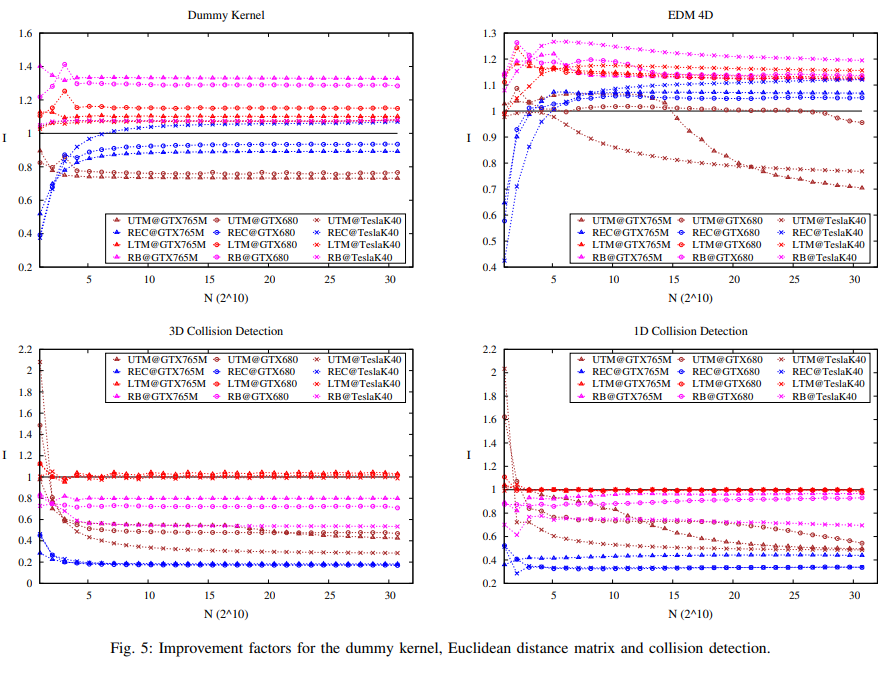
\includegraphics[width=\textwidth]{figures/fig5.png}
  \caption{Factores de mejora para el dummy kernel, la matriz de distancias
           euclidianas y la detección de colisiones.}
  \label{fig:fig5}
\end{figure*}

En cada gráfico se representa el rendimiento de las cuatro estrategias como
diferentes colores de líneas discontinuas, mientras que el símbolo de punto
corresponde a la diferente GPU elegida para esa prueba. El rendimiento de cada
estrategia de mapeo se da en términos de su factor de mejora $I$ respecto a la
estrategia BB (es decir, la línea horizontal negra y sólida fijada en $I = 1$).
Los valores ubicados sobre la línea horizontal representan una mejora real,
mientras que las curvas que caen bajo la línea horizontal representan una
ralentización respecto a la estrategia BB.

Para la prueba del dummy kernel observamos que la estrategia RB es la más
rápida, logrando hasta un 33\% de mejora respecto a BB al ejecutarse en el
GTX~765M. LTM ocupa el segundo lugar logrando una mejora estable del 18\% al
ejecutarse en el GTX~680. Las estrategias REC y UTM se desempeñaron más
lentamente que BB para todo el rango de $N$. Notamos que esta prueba
ejecutándose en el Tesla~K40 no proporciona ninguna diferencia de rendimiento
clara entre las estrategias de mapeo una vez que $N > 15000$, ya que todas
convergen a un 7\% de mejora respecto a BB.

Para la prueba EDM, observamos que RB es nuevamente el mapa más rápido
logrando una mejora de hasta 28\% respecto a BB al ejecutarse en el GPU
Tesla~K40. En segundo lugar está LTM con una mejora estable del 18\% y en
tercero el mapa REC con una mejora que alcanza hasta el 12\% para el $N$ más
grande. El rendimiento de la estrategia UTM es inferior a BB e inestable para
todos los GPUs. En este punto, hay que considerar que UTM fue diseñado para
funcionar en el rango $N \in [0, 3000]$, donde en realidad sí se desempeña
mejor que BB ofreciendo hasta un 4\% de mejora sobre BB. Para esta prueba,
las diferencias de rendimiento sí se manifestaron para todos los GPUs, incluso
en el Tesla~K40.

Para la prueba de detección de colisiones hemos incluido dos casos: detección
de colisiones 3D y 1D. De todas las estrategias de mapeo, solo LTM logra
desempeñarse mejor que BB, ofreciendo una mejora de hasta 7\%. De hecho, el
escenario de rendimiento cambia drásticamente en presencia de un patrón de
acceso a memoria diferente como la memoria compartida; la estrategia RB, que
era la mejor en memoria global, ahora se desempeña más lentamente que BB. El
caso es similar con el mapa REC, que ahora se desempeña mucho más lento. Es
importante mencionar que el mapa UTM es la única estrategia que no puede usar
un patrón de memoria compartida 2D porque el mapeo funciona en el espacio
lineal de threads. Para valores bajos de $N$, UTM logra una mejora del 100\%
debido al diferente enfoque de memoria utilizado. Sin embargo, a medida que
$N$ crece, su rendimiento es superado por el resto de las estrategias que usan
memoria compartida. Para el caso de la detección de colisiones 1D, los
resultados no son tan beneficiosos para las estrategias de mapeo y en el caso
de LTM el rendimiento está en el límite de no convertirse en una mejora. Los
resultados 1D muestran que en dimensiones bajas los beneficios de una
estrategia de mapeo pueden no ser tan buenos como en dimensiones altas.

% ---- Tabla I ----
\begin{table}[H]
\centering
\caption{Hardware utilizado en los experimentos.}
\label{tab:hardware}
\small
\begin{tabular}{ll}
\toprule
\textbf{Componente} & \textbf{Descripción} \\
\midrule
CPU  & i7-3770K @ 3.50\,GHz \\
RAM  & 32\,GB DDR3 1333\,MHz \\
GPU1 & GTX~680 (GK104, 2\,GB, 1536 núcleos) \\
GPU2 & GTX~765M (GK106, 2\,GB, 768 núcleos) \\
GPU3 & Tesla K40 (GK110, 12\,GB, 2880 núcleos) \\
API  & CUDA 5.5 \\
\bottomrule
\end{tabular}
\end{table}

% ============================================================
\section{Conclusiones}
\label{sec:conclusions}

Hemos estudiado los beneficios de los mapas GPU para problemas de dominio
triangular, alias td-problems. Estos mapas permiten el uso de un espacio de
cómputo más pequeño comparado con la estrategia de bounding box (BB) para
resolver un problema. Al usar un espacio de cómputo más pequeño, el número de
threads innecesarios se reduce y el kernel de GPU puede ejecutarse más rápido.
Nuestro mapa GPU propuesto, denominado LTM por lower triangular map, usa una
función $g(\lambda)$ para mapear el espacio de cómputo a cualquier td-problem.
La principal ventaja de LTM es que funciona en el espacio de bloques, no
afectando la organización de threads y permitiendo tamaños de problema de al
menos $N \in [0, 30720]$, que es diez veces el rango logrado en el
upper-triangular map (UTM) \cite{ref1}. Es importante mencionar que el tamaño
del problema debe ser lo suficientemente grande para generar más bloques que el
número de bloques que la GPU puede manejar en paralelo. Asumiendo un warp de 32
threads, un valor de $N \geq 800$ ya genera más del doble del número de bloques
en paralelo para cualquiera de los GPUs que usamos. Para valores más pequeños
de $N$, la estrategia BB seguirá siendo útil.

Al comparar todas las estrategias de mapeo bajo las mismas pruebas de
rendimiento, encontramos que el rectangular box (RB) y LTM son las mejores
estrategias de mapeo para un problema basado en memoria global como EDM,
logrando un 28\% y un 18\% de mejora, respectivamente. La estrategia
recursive partition (REC) logró proporcionar hasta un 12\% de mejora para el
problema de memoria global. La estrategia UTM logró menor rendimiento que el
método BB y no pudo proporcionar resultados exactos cuando $N > 3000$. Para
la detección de colisiones con memoria compartida encontramos que ninguna
estrategia excepto LTM logró superar a BB, en un 7\%. La razón por la que
LTM aún pudo proporcionar una mejora bajo un patrón de acceso a memoria
diferente es que LTM mapea en el espacio de bloques, por lo que no compromete
la organización de threads. Los beneficios del mapeo en el espacio de bloques
se manifiestan mejor bajo algoritmos de memoria compartida o técnicas de
engrosamiento de threads \cite{ref13}.

La implementación de la estrategia LTM es extremadamente corta en código y
totalmente desvinculada del problema, lo que facilita su adopción. Al elegir
la mejor implementación de raíz cuadrada, encontramos que la raíz cuadrada
recíproca fue la opción más conveniente para GPUs GK104 y GK106, como el
GTX~680 y GTX~765M, respectivamente. Al ejecutar el mapa LTM en el GPU
Tesla~K40 de Nvidia, que es una arquitectura GK110, encontramos que el cómputo
de la raíz cuadrada puede realizarse simplemente usando la función predeterminada
\texttt{sqrtf(x)} sin ninguna penalización en el rendimiento. Esto hace que la
implementación de LTM sea aún más simple.

El rendimiento de las estrategias de mapeo para td-problems sigue variando
dependiendo del GPU usado y de la manera en que se accede a la memoria, lo que
dificulta elegir el mejor mapa. Sin embargo, hemos encontrado algunos patrones
de rendimiento importantes entre nuestros resultados: los mapas RB y LTM son
buenos para problemas de memoria global, mientras que el mapa LTM es el único
bueno para un problema basado en memoria compartida. Este escenario pone a LTM
en ventaja sobre los otros mapas, ya que es la única estrategia que puede
funcionar tanto para problemas basados en memoria global como compartida.

% ============================================================
\section*{Agradecimientos}

Los autores desean agradecer a CONICYT por financiar el programa de doctorado
de Crist\'obal A.\ Navarro. Este trabajo fue parcialmente apoyado por el
proyecto FONDECYT No.\ 1120495.

% (figuras ubicadas inline en el texto)

% ============================================================
\bibliographystyle{plain}
\bibliography{references}

\end{document}
